\subsection{Discrete Multi-Marginal Optimal Transport}

%The natural next step from above is an extension when we have an arbitrary number of $d>2$ distributions. 
%A limitation of t
The foregoing approach 
%is that it 
applies only to $d=2$ distributions, namely $p_1$ and $p_2$. We briefly review the extension 
%of the above idea 
to $d>2$ distributions; 
%. The optimal transport 
the literature calls this \textit{multi-marginal optimal transport (MMOT)}.%, with similar subproblems following problem and cost-specific assumptions a la Kantorovich and Monge. Here we focus on the discrete setting.
% \vikas{give the reader a sense of whether this is still background material and/or where this is going.}

\begin{definition}[Discrete Multi-Marginal Optimal Transport (d-MMOT)]\label{def:dmmot}
Let $p_1, \ldots, p_d\in\RR^n_{+}$ be discrete probability distributions. %Then, $e'p_i=1$ for all $i\in[d]$. % with each $p_i \in \Delta^n$, where $\Delta^n$ is the $n$-dimensional simplex. 
%Let $c_d : \cX^d \rightarrow \RR_{\ge 0}$. 
Let $C_d : \RR^{n^{d}}\rightarrow \RR_{+}$. 
The discrete multi-marginal optimal transport problem (d-MMOT) can be written as
\begin{align*}%\label{eq:dmmot}
    %&\underset{{X \in \cX^d}}{\textrm{minimize}}\quad C_d(X) \\
    &\underset{{X \in \RR^{n\times \cdots \times n}}}{\textrm{min}}\quad C_d(X) \quad \textrm{s.t.}\quad X_i = p_i,\ (\forall i\in [d]),
\end{align*}
where $X_i \in \RR^n$ is the $i$-th marginal of  $X \in \RR^{n\times \cdots \times n}=\RR^{n^{d}}$.
\end{definition}
Following the original formulation \citep{kantorovich1942}, we will restrict the cost function $C_d(\cdot)$ to the linear map, $C_d(X) \coloneqq \langle c, X \rangle_{\otimes}$, where $c \in \RR_{+}^{n\times \cdots \times n}$ is nonnegative.
%The sequel will focus on the following form of the d-MMOT problem.
Here, the d-MMOT is the LP,
\begin{align}\label{eq:gemd}\begin{aligned}
    \underset{x\in\RR^{n^{d}}_{+}} {\textrm{min}}
    \sum_{i_1,\ldots,i_d} c(i_1,\ldots, i_d)\, x(i_1,\ldots,i_d) \quad \textrm{s.t.}
    \sum_{i_2,\ldots,i_d} x(i_1,\ldots,i_d) &= p_1(i_i), (\forall i_1\in[n])\\
    % &\sum_{i_1,i_3\ldots,i_d} c(i_1,\ldots, i_d)x(i_1,\ldots,i_d) = p_2(i_2),\ (\forall i_2\in[n])\\
    \qquad\vdots\\
    \sum_{i_1,\ldots,i_{d-1}} x(i_1,\ldots,i_d) &= p_{d}(i_{d}), (\forall i_d\in[n]).
    \end{aligned}
\end{align}
This linear program is central to the regularization schemes that are discussed below.
\section{Efficient d-MMOT Computation}
The linear d-MMOT problem (\ref{eq:gemd}) suffers from the curse of dimensionality: the LP has $n^d$ variables, and even modest choices of $n$ and $d$ can result in a LP with billions of variables, making standard LP solvers inapplicable.
%Traditional linear programming solvers such as interior point methods have been studied in the two-dimensional context, but the MMOT setting does not allow a direct extension given the exponential dependence on $d$. 
Alternatively, specific algorithms have been proposed  \citep{benamou2015iterative}, and 
relaxations via entropic regularization have become more widespread, with very recent extensions to the d-MMOT setting \citep{tupitsa,mmotcuturi}. 

% Putting aside the computation of the dMMOT objective,
% in practical applications its often the case that moving input distributions closer or further from each other requires minimizing or maximizing the objective. Define an arbitrary distance among distributions as $\phi(p_1, \ldots, p_d)$. If this distance is defined as the objective in \eqref{eq:gemd},
% then minimizing the distance among distributions in this form requires bilevel optimization.
% Of course we can set all distributions to be the same for the problem to minimized,


In practice, the cost $c$ in (\ref{eq:gemd}) typically takes one of two forms. In the case where the distributions $p_1, \ldots, p_d$ are over categorical variables, the cost is typically defined as $c(i_1, \ldots, i_d) = 0$ when $i_1 = \cdots = i_d$ and $1$ otherwise.
However, and importantly, if the distributions $p_i$ are histograms over some ordinal or discretized space, 
the cost typically has a structure 
closer to that of a ``tensorized'' distance, characterized by the {\em Monge} property.
%\ronak{emphasize this, it is key to distinguish our construction, maybe add motivation in intro re this}
\begin{definition}[Monge Property]
A tensor $c$ is Monge if for all valid $i_1, \ldots i_d$ and $j_1, \ldots, j_d$, 
%$1 \leq i_1 \leq j_1 \leq n$, $1 \leq i_2 \leq j_2 \leq n$, $1 \leq i_d \leq j_d \leq n$,
\begin{align}
c(s_1, \ldots, s_d) + c(t_1, \ldots t_d) \leq c(i_1, \ldots i_d) + c(j_1, \ldots, j_d)
\end{align}
where $s_k = \min(i_k, j_k)$ and $t_k = \max(i_k, j_k)$.
\end{definition}
Our focus is on a specific cost, which is known to be Monge: $c(i_1,i_2,\ldots,i_d)\coloneqq \max{\{i_k:k\in[d]\}} - \min{\{i_k:k\in[d]\}}$. When $d=2$, this cost reduces to $c(i_1,i_2)=|i_1-i_2|$, which agrees with the classical EMD cost. This choice of $c$ is called the {\em generalized EMD cost}.


%\ronak{this is not explained below, a sentence here in place suggesting how its used in histograms/etc would  be better}

% While the Monge restriction may seem ``nicer" compared to arbitrary nonnegative costs, it is not yet clear how this can be leveraged for efficient computation. 
% The Monge cost does not in itself provide nicer properties to existing methods for multi-marginal optimal transport,
% the program suffers from the curse of dimensionality.
% If $d$ histograms with $n$ bins are being compared, the decision variable of the program still lies in $\RR^{n^{d}}$, which can be very large even if both $d$ and $n$ are modest (say $n=d=10$). 
% To progress in any direction, it is necessary for us to identify a method for taking advantage of this structure in an efficient manner.

%\vikas{the following needs attention. We should think of how to provide some daylight -- because as written, it seems what a reader may call a ``direct application''.}
\begin{remark}Limiting our attention to this cost is not as restrictive as it may appear. 
Indeed, \cite{BEIN199597} shows that the optimal solution to the LP (\ref{eq:gemd}) is independent of the cost, as long as it is Monge.
Additionally, when $c$ is the generalized EMD cost, \cite{kline2019properties} describes a greedy algorithm that solves both (\ref{eq:gemd}) and its dual (\ref{eq:dualgeneralemd}) in linear time. 
% They present an algorithm (presented in Algorithm~\ref{alg:primaldual})
% and constructs a theoretical and algorithmic framework for solving the discrete MMOT.
% Particularly,
% \ronak{key results from kline19, complexity, short description of results}
%\begin{remark}
It is also shown that the optimal objective value is a continuous nonnegative function of each probability distribution $p_j$ (i.e., small changes in one distribution cause small changes in the objective value). Continuity is critical for numerical stability.  Next, when $c$ is the generalized Earth Mover's array, the optimal objective value vanishes if and only if $p_i=p_j$ for all $i,j\in[n]$. 
%\end{remark}
\end{remark}
This {\em separability} property is useful in applications where we wish to iteratively ``step towards'' the barycenter of a set of distributions, see Figure \ref{fig:min_demd}.
%{\color{blue} This typically would happen in an {\em outer} loop when training a deep neural network. }
In order to step towards {red arrows)} a barycenter, we  require a descent direction.  %This is the next result.
%While we can directly push them all towards an arbitrary point in the simplex (e.g., uniform, barycenter), it would be better if we could naturally move towards a point that is close, in some sense, to the initial distributions.
% is relevant since our goal is to regularize the model in a way that favors equi-distribution of mass across multiple probability densities.
We observe that the following  result gives us  this functionality.

% We can also write the dual linear program.
% \begin{alignat}{2}\label{eq:dualgeneralemd}\begin{split}
% &\underset{z_j\in\RR^n, j\in[d]}{\textrm{maximize}}\qquad\sum_{j} x_j'z_j\\
% &\textrm{subject to}\qquad z_{1}(i_1)+\cdots+z_{d}(i_{d})\leq c(i_1,\ldots,i_{d}),\end{split}
% \end{alignat}
% where the indices in the constraints include all $i_j\in[n]$, $j\in[d]$.

% The following result will make use of the dual linear program.  Before stating the theorem, we introduce some notations. Given distributions $p_1,p_2,\ldots,p_d\in\RR^{n}$ with $e'p_j=1$ for all $j\in[d]$, denote by $\phi(p_1,\ldots,p_d)$, the optimal objective value of the LP in (\ref{eqn:gemd}). Denote by
% \begin{align*}z^*=(z_1^{*}, z^*_2,\cdots,z^*_{d}),
% \end{align*}
% an optimal solution to the dual program~(\ref{eq:dualgeneralemd}).
\begin{theorem}
The dual linear program of the d-MMOT problem (\ref{eq:gemd}) is
\begin{alignat}{2}\label{eq:dualgeneralemd}
\begin{split}
\underset{z_j\in\RR^n, j\in[d]}{\textrm{maximize}}\qquad\sum_{j} p_j'z_j 
\qquad \textrm{subject to}\qquad z_{1}(i_1)+\cdots+z_{d}(i_{d})\leq c(i_1,\ldots,i_{d}),
\end{split}
\end{alignat}
where the indices in the constraints include all $i_j\in[n]$, $j\in[d]$.
Denote by $\phi(p_1,\ldots,p_d)$, the optimal objective value of the LP in (\ref{eq:gemd}). Let $z^*$ be an optimal solution to the dual program~(\ref{eq:dualgeneralemd}).
Then,
% In the established notation, the following two claims hold. First,
\begin{align*}
\nabla \phi(p_1,\ldots,p_{d}) = z^*, 
%\end{align*}
~~\text{and for any $t\in \RR$,}~~
%\begin{align*}
\phi(p_1,p_2,\ldots,p_{d}) = \sum_{j}p_j'
(z_j^* + t\, \eta),
\end{align*}
where $\eta\coloneqq (z_1^{*}(n)\,e, z^*_1(n)\,e, \cdots, z^*_{d}(n)\,e)$.
\label{thm:dualgrad}
\end{theorem}
\begin{proof}
The main observation invokes perturbation analysis \citep{mangasarian1979nonlinear,ferris1991finite} of LPs to assert that, under mild uniqueness conditions, small changes to a LP's input data does not change its optimal solution. The full proof is in Appendix~\ref{sec:app-proof}.
\end{proof}
\begin{remark} The first part of this result provides what we require: a direction of descent. 
Thus, if we can solve the d-MMOT problem and also find the optimal solution to its dual, 
then we can step (or move) our distributions in the opposite direction of the dual variables
to push them together, see Figure~\ref{fig:min_demd}.
The second claim is somewhat technical, and reconciles particular affine shifts that result in equivalent objective values.
\end{remark}

% The second claim, which is rather technical, requires some motivation/explanation for why it was included. 
% We observed empirically that solutions yielded by either autograd or by numerical approximations differed from the solutions yielded by the greedy algorithm that we employ. 
% But the difference was, in all cases, inconsquential: the dual objective functional, evaluated on both vectors agreed, and in all examples tested, the difference equaled a constant factor times the vector $\eta$ that is stated in the theorem.
\subsection{Optimization of d-MMOT}\label{sec:dual}

\paragraph{Setup.} 
We can now instantiate d-MMOT as an add-on term in a standard machine learning formulation. Concretely, it can be positioned alongside typical learning losses $L(f(x),y;\theta)$ to encourage minimizing distances among $d$ different distributions $g_i\in G, i \in [d]$, $\text{d-MMOT}(f(x),g;\theta)$, i.e., 
\begin{align}
\min_{\theta} L(f(x),y;\theta) + \text{d-MMOT}(f(x),g;\theta).
\end{align}
Within a deep neural network (DNN) architecture, as in some of our experiments,  
several properties of the d-MMOT module are useful:
our results above naturally provide clean operations for computing both the required objective in the ``forward'' pass and gradients in the ``backward'' pass.


\begin{figure}
    \centering
    %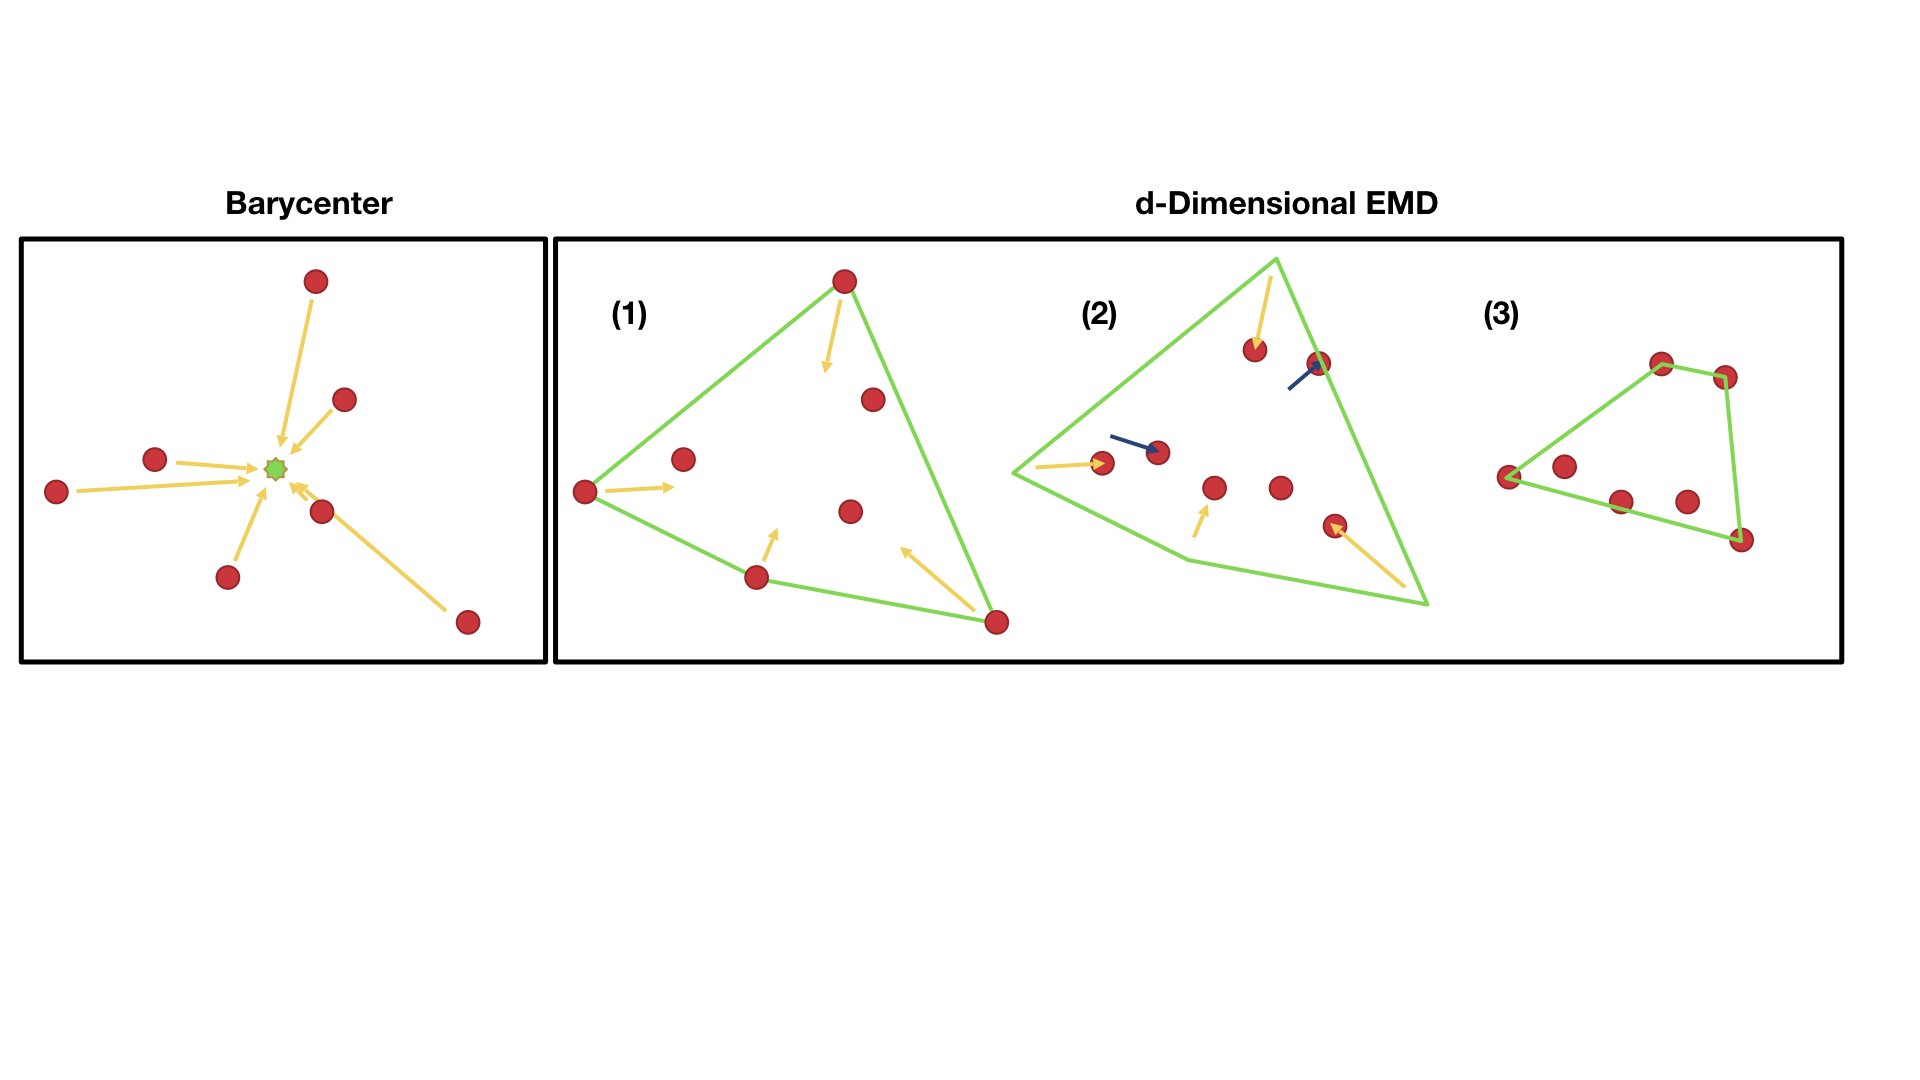
\includegraphics[trim={0 14.5cm 2cm 5cm},clip,width=\textwidth]{6_demd/figs/demd_abstract.png}
    % 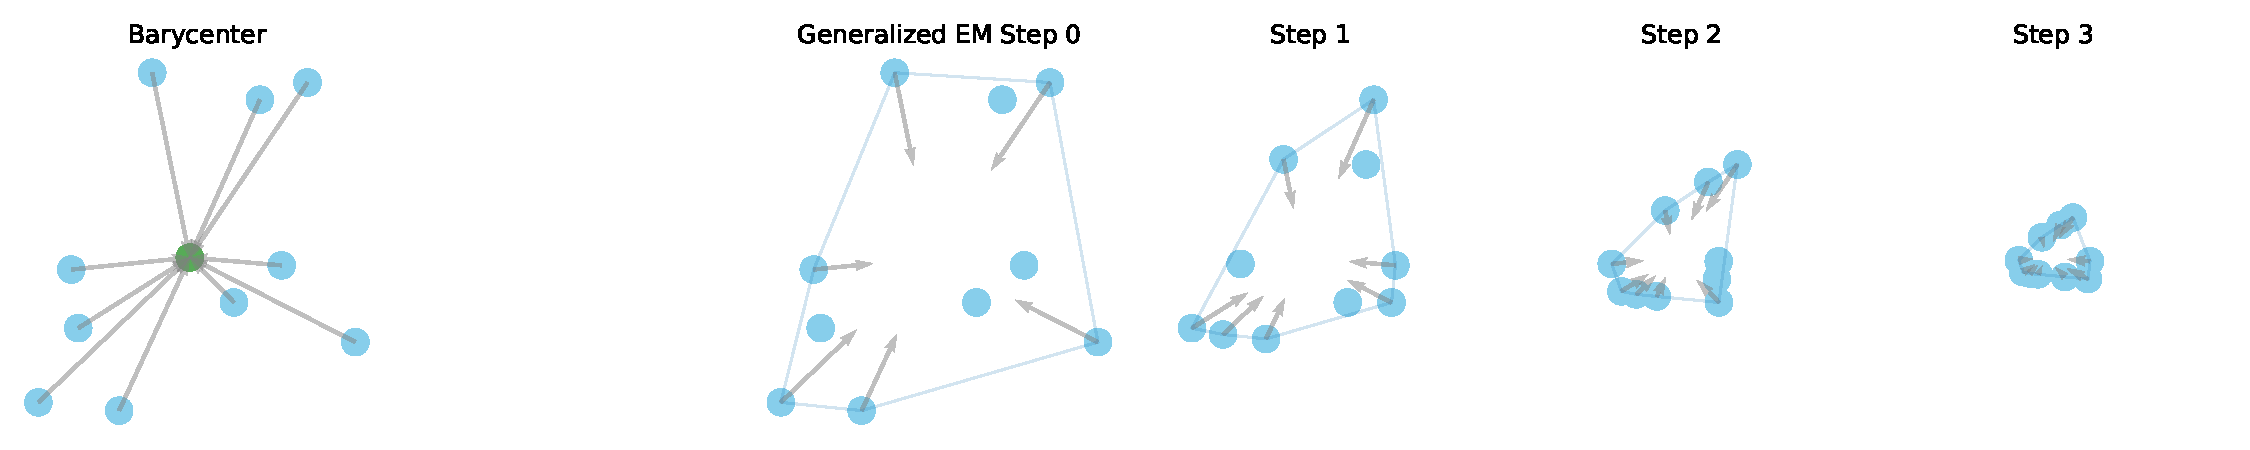
\includegraphics[width=0.95\textwidth]{6_demd/figs/bary-gem-step.pdf}
    %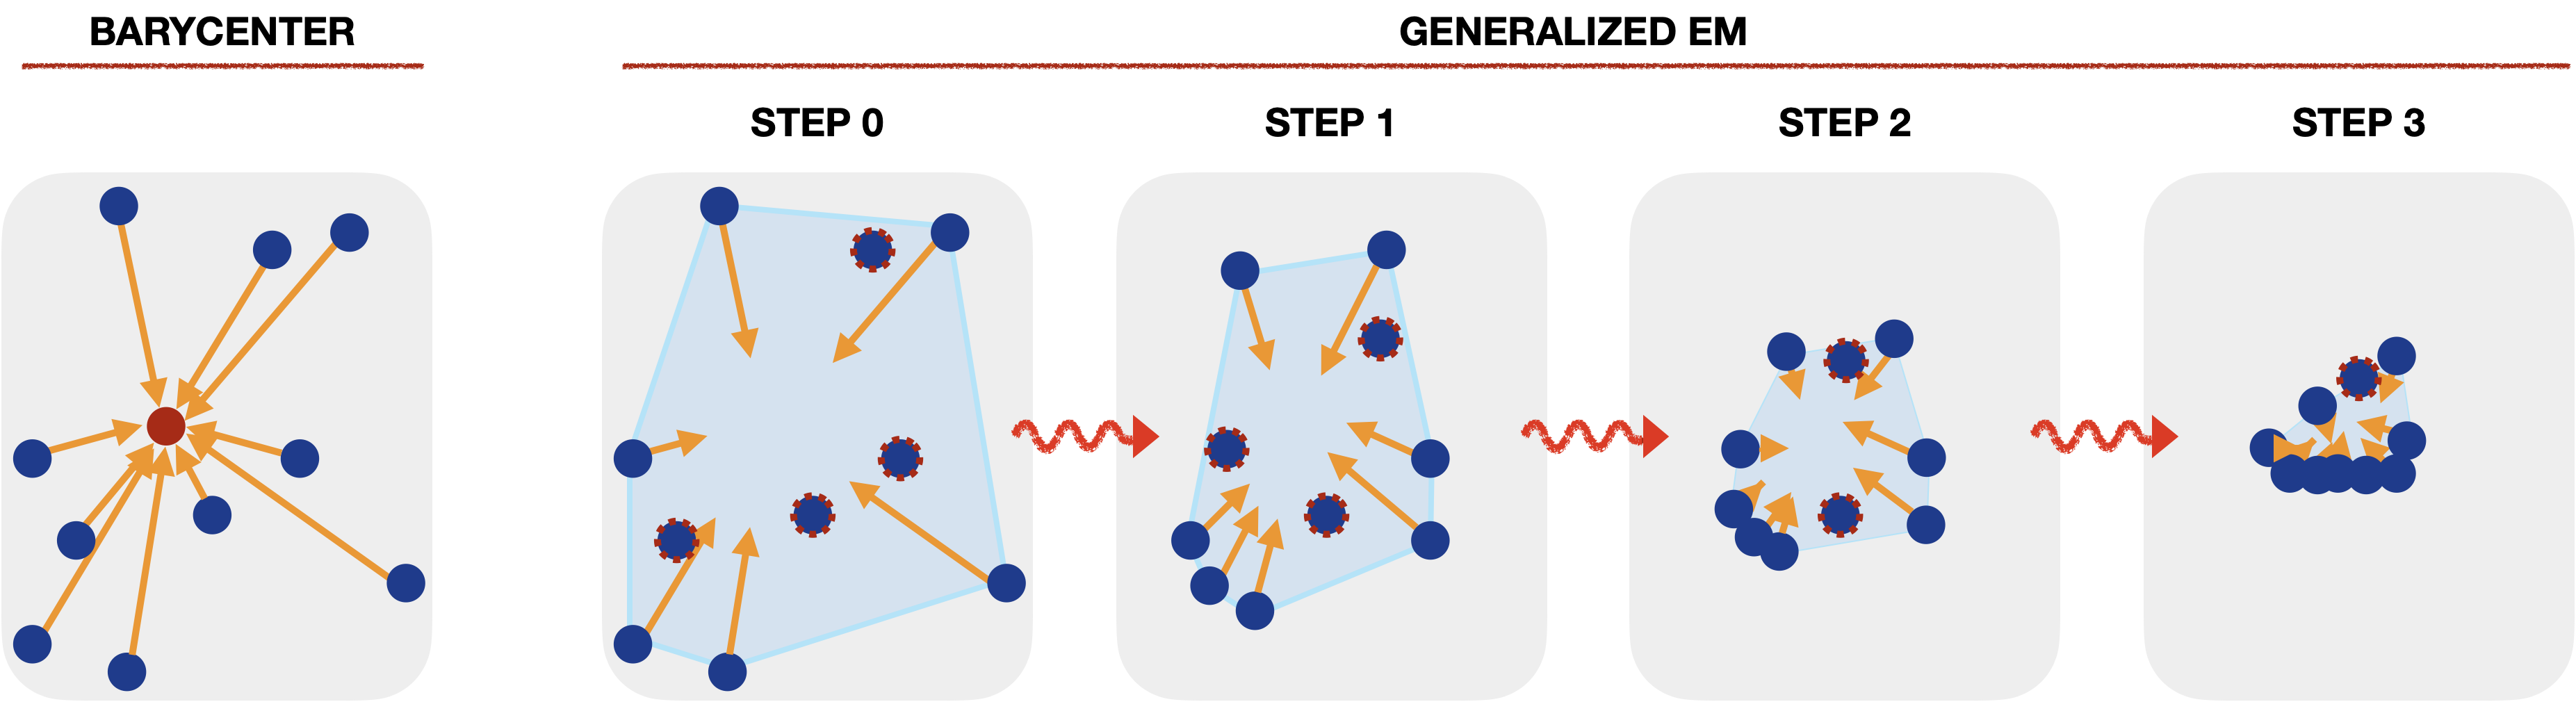
\includegraphics[width=0.9\textwidth]{6_demd/figs/demd_hull_new.png}
    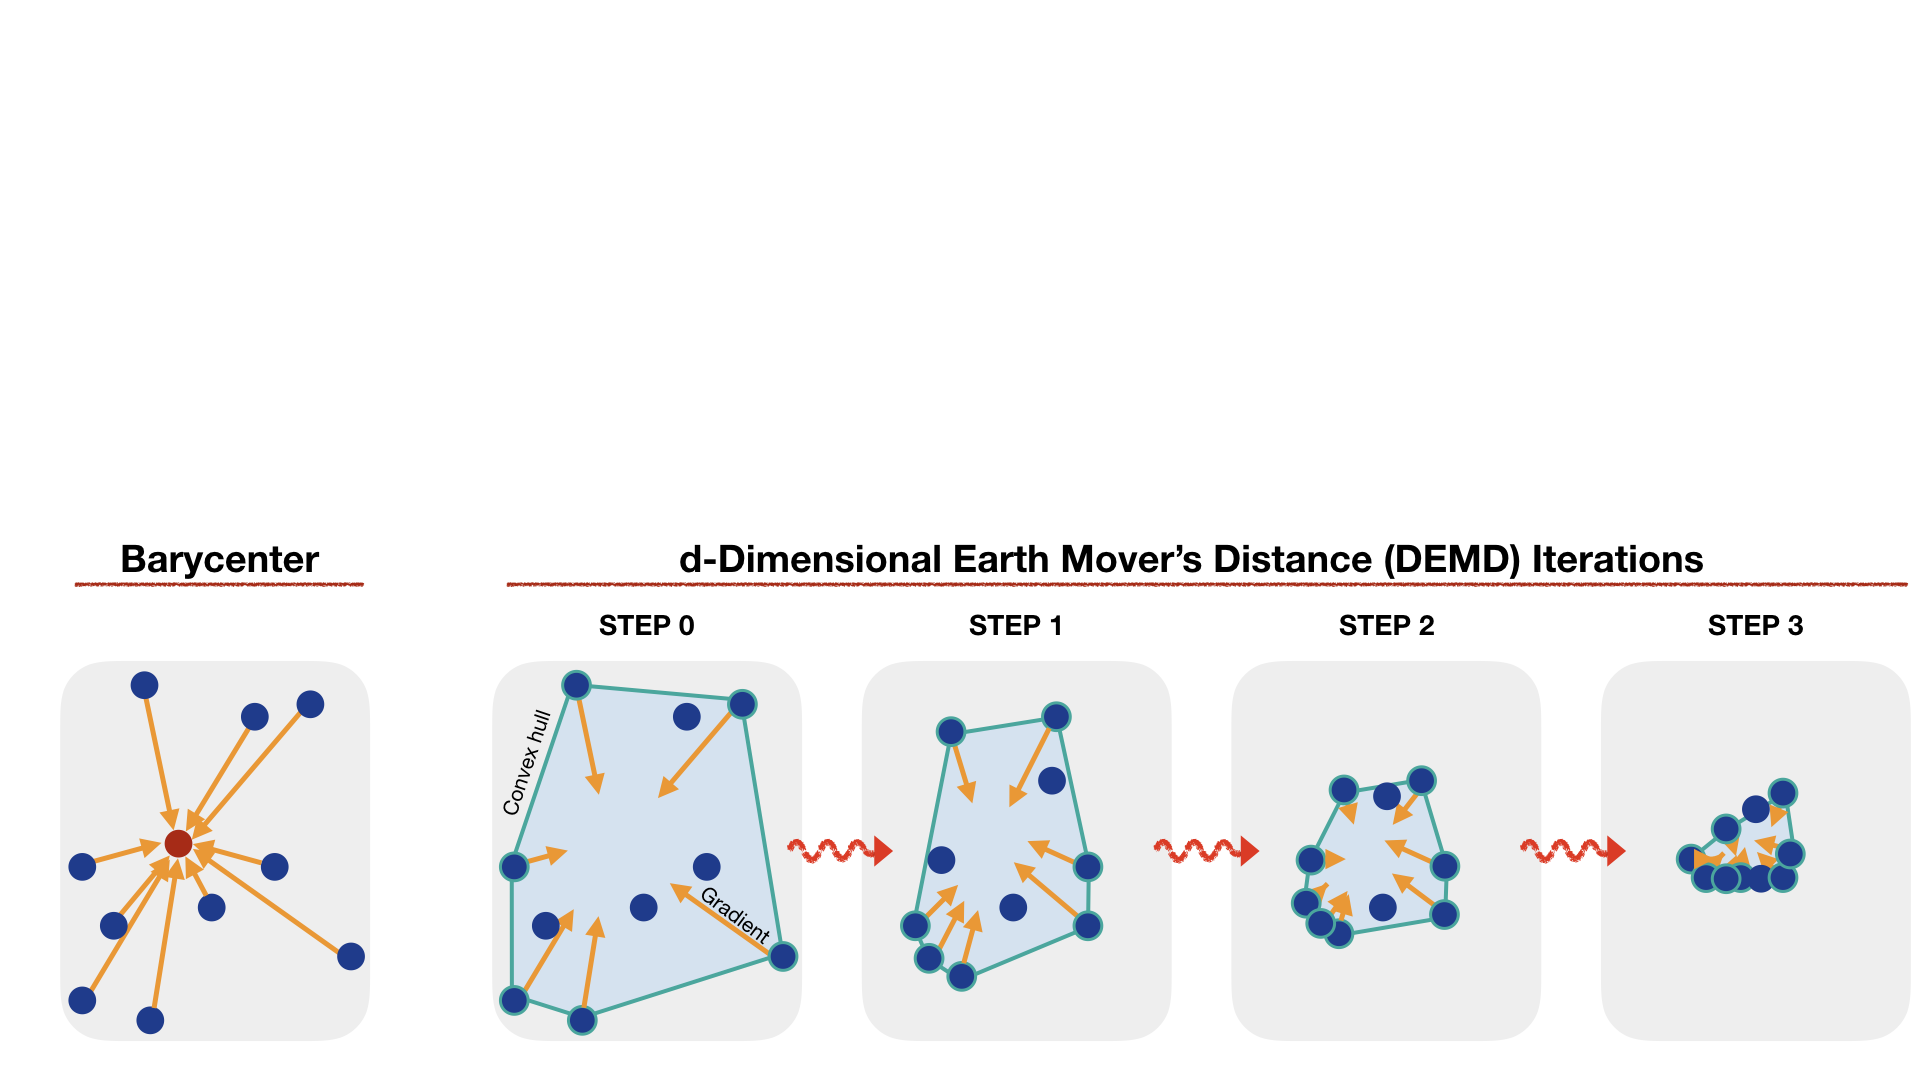
\includegraphics[trim={2cm, 0, 0, 18cm},clip,width=0.9\textwidth]{6_demd/figs/demd_hull_v3.png}
    \caption[Visualizing steps withing the d-MMOT minimization]{({\em Left}) Barycenter methods identify a center (red circle) and transport \textit{all} distributions (blue circles) toward that center along the coupling path (yellow). ({\em Right}) Our DEMD approach identifies ``support" distributions that lie on the convex hull (outlined circles),  and only those distributions are moved in a direction that decreases the Generalized EMD objective.}
    \label{fig:min_demd}
\end{figure}

% \subsection{Solving the dMMOT program and its dual}\label{sec:dual}
% JK: this paragraph interrupts the flow
%Using either the iterative Bregman or Sinkhorn-style methods within an outer optimization is  impractical: invoking an interior point solver at each outer iterate explodes an already exponentially large problem, and methods extending two-dimensional entropic relaxations such as unrolling add significant complexity and require approximate solutions.

% Linear program solvers are now a  mature technology,  with polynomial-time guarantees for solution accuracy.
% Despite this, they are unsuitable as the engine that solves the programs of our intended use-case, namely regularizing a network model. 
% Our intent is to have the ability to embed a process that solves an instance of (\ref{eqn:gemd}) and its dual repeatedly during network training.  One reason standard methods are too slow for this is that the programs themselves can be quite large: recall that the cost functional is a dense, rank-$d$ tensor. We note 
% however that there is recent progress towards differentiable LP modules  \cite{meng2020differentiable,NEURIPS2020_6bb56208}. 


% \begin{remark}
% % While recent progress has been made towards differentiable LP modules \citep{meng2020differentiable,NEURIPS2020_6bb56208},
% % here we instead observe that 
% Indeed, these approaches are a necessary path forward given the problem as written,
% where infeasibility is proven for the unregularized formulation (Theorem 3.3 in \cite{mmotcuturi}).
% Notably, their proof follows directly by identifying a form of the cost tensor $C$ such that a reduction to a matching problem leads to a contradiction in theoretical hardness.
% % \vikas{some form of the following sentence needs to be positioned a bit earlier and perhaps repeated here. We need to contrast it with the literature. Is this novel/new etc.}
% In what follows we identify a specific form of the cost tensor $C$ that not only allow for a tractable algorithm, but also has key properties that can be exploited in downstream applications.
% \end{remark}


% In practice, the form of the cost $C$ typically takes two forms. In the case where the distributions $p_1, \ldots, p_d$ are over categorical variables, the cost is typically defined as $c(i_1, \ldots, i_d) = 0$ when $i_1 = \cdots = i_d$ and $1$ otherwise.
% On the other hand, if the distributions $p_i$ are histograms over some ordinal or discretized space, 
% the cost typically follows a structure 
% closer to that of a metric.
% Cost tensors that form these sorts of metrics can be characterized by a tensor form of a distance. \ronak{emphasize this, it is key to distinguish our construction, maybe add motivation in intro re this}
% \begin{definition}[Monge Array]
% A tensor $C$ is Monge if for all valid $i_1, \ldots i_d$ and $j_1, \ldots, j_d$, 
% %$1 \leq i_1 \leq j_1 \leq n$, $1 \leq i_2 \leq j_2 \leq n$, $1 \leq i_d \leq j_d \leq n$,
% \begin{align}
% c(s_1, \ldots, s_d) + c(t_1, \ldots t_d) \leq c(i_1, \ldots i_d) + c(j_1, \ldots, j_d)
% \end{align}
% where $s_k = \min(i_k, j_k)$ and $t_k = \max(i_k, j_k)$.
% \end{definition}

% While the Monge restriction may seem ``nicer" compared to arbitrary nonnegative costs, it is not yet clear how this can be leveraged for efficient computation. 
% The Monge cost does not in itself provide nicer properties to existing methods for multi-marginal optimal transport,
% the program suffers from the curse of dimensionality.
% If $d$ histograms with $n$ bins are being compared, the decision variable of the program still lies in $\RR^{n^{d}}$, which can be very large even if both $d$ and $n$ are modest (say $n=d=10$). 
% To progress in any direction, it is necessary for us to identify a method for taking advantage of this structure in an efficient manner.

% \vikas{the following needs attention. We should think of how to provide some daylight -- because as written, it seems what a reader may call a ``direct application''.}
% Recent work by
% \cite{kline2019properties} leverages the properties of the dMMOT problem with this cost, albeit with a focus on the specific $d$-dimensional earth mover's construction. Interestingly, the algorithm and analysis therein can be leveraged to solve the d-MMOT problem.
% They present an algorithm (presented in Algorithm~\ref{alg:primaldual})
% and constructs a theoretical and algorithmic framework for solving the discrete MMOT.
% Particularly,
% \ronak{key results from kline19, complexity, short description of results}

\paragraph{Using the primal and dual variables.}  If the optimal objective value of (\ref{eq:gemd}) serves in regularizing a deep neural network, then we can train the network as follows. %this means can compute the objective value during a the forward pass
%The first issue is trivial to implement within standard neural network frameworks. 
% During the forward pass, one can compute the EMD term using the primal/dual greedy algorithm of \cite{kline2019properties}, with one simple modification:  prior to returning, the dual solution variables are stored for use during the backward pass. 
During the forward pass, i.e., computing the d-MMOT objective, we can employ a version of the aforementioned primal/dual algorithm that solely computes the function $\phi$ and stores the dual variables $z$.
As backpropagation proceeds, when the EMD module encounters an incoming gradient, it is simply multiplied by the stored dual variables (see Theorem~\ref{thm:dualgrad} and Algorithm~\ref{alg:demdFunc}). We call our procedure the $d$-dimensional Earth Mover's Distance, or in short,\textit{ the DEMD algorithm}. 
\begin{algorithm}
	\caption{ \label{alg:demdFunc} $d$-Dimensional Earth Mover's Distance (DEMD)}
	\SetAlgoLined
	\DontPrintSemicolon
	\SetKwFunction{FVar}{Forward}
	\SetKwProg{Fn}{Function}{:}{}
	\Fn{\FVar{$p_1, \ldots, p_d$}}{
		Compute $\sum s_k t_k$ and $(z_1,\ldots,z_d)$ via \cite{kline2019properties}. \\
		Save $(z_1,\ldots, z_d)$. \\
		\KwRet{$\sum_k s_k t_k$}
	}
	\SetKwFunction{FCore}{Backward}
	\SetKwProg{Gn}{Function}{:}{}
	\Gn{\FCore{$\text{gradOutput}$}}{
		Load $(z_1,\ldots, z_d)$ \\
		\KwRet{$(z_1,\ldots, z_d)\cdot \text{gradOutput}$}
	}
\end{algorithm}


\paragraph{Complexity.} Computing the DEMD distance in the forward pass is exactly $O(nd)$: linear in the number of distributions and number of bins. This property follows directly from the algorithm, needing only a single pass through all of the data. \cite{BEIN199597} provides this result for greedy algorithms that solve OT programs as in Definition~\ref{def:dmmot}. In contrast to methods that derive gradients via entropic regularization schemes, i.e., relaxations of the optimal transport problem \citep{diffpropsinkwass,difftopkOT,quantnorm}, this approach solves the distance computation exactly in linear time.
This analysis is not only provided by the theory in prior work, but is also explicit in the number of iterations defining our algorithm (see Appendix~\ref{sec:suppdemd} for more details).
For minimizing the DEMD (computing the updates, i.e., red arrows in Figure~\ref{fig:min_demd}), a convergence analysis would follow from the properties of the optimization scheme chosen. Our tool can be dropped in exactly as any other module in modern learning applications (using the observation that gradients are easily computed, i.e., $O(1)$ time to read stored dual variables). %Convergence analysis would follow from the optimization method chosen (SGD, ADAM, etc.).
%}

% It is this construction that we take advantage of and expand upon. 
% \vikas{pose the issue/question first. Then say that we will start from Kline, which we observe can be part of a solution.}

% In this section, we make precise the generalization of the classical Earth Mover's distance. We also state Theorem~\ref{thm:dualgrad}, which establishes that a solution to the generalized linear program's dual equals the gradient of the optimal objective value of the primal linear program.

% \subsection{Multi Marginal Optimal Transport}

% Given a collection of probability distributions $P_1, \ldots, P_m$ over $\cX$, and the cost function $c_m : \cX^m \rightarrow \RR_{\ge 0}$, the multi-marginal optimal transport problem is to minimize $\EE[c_m(X_1,\ldots, X_m)]$ over all couplings of $P_1, \ldots, P_m$, or $X_i \sim P_i$.

% \begin{definition}
% Let $p_1, \ldots, p_m$ be discrete distributions, with each $p_i \in \Delta^n$, where $\Delta^n$ is the $n$-dimensional simplex. Let $c_m : \cX^m \rightarrow \RR_{\ge 0}$. Then the \textbf{discrete multi-marginal optimal transport problem} is
% \begin{align}
%     &\min_{X \in \cX^m}\quad c_m(X) \\
%     &s.t.\quad X_i = p_i \ \forall i
% \end{align}
% \end{definition}

% \begin{proposition}
% Restrict the cost $c_m$ above to be Monge. Then the \textbf{\textit{discretized} multi-marginal optimal transport} is equivalent to the $m$-dimensional earthmover's distance.
% \end{proposition}

% \begin{proposition}
% The d-MMOT or DEMD problem is efficiently solvable.
% \end{proposition}

% \begin{proposition}
% The algorithm results in gradients readily available...
% \end{proposition}


% Before stating the generalized formulation, several points are worthwhile to note. First, the generalized description contains the classical Earth Mover's distance when pairs of distributions are being compared. Second, the generalized program suffers from the curse of dimensionality. If $d$ histograms with $n$ bins are being compared, the decision variable of the program lies in $\RR^{n^{d}}$, and $n^d$ can be very large even if both $d$ and $n$ are modest (say $n=d=10$). 
% However,  this is not an issue in practice: both primal and dual linear programs can be solved using an extremely efficient greedy algorithm, and the decision variable is extremely sparse.

% The classical EMD in (\ref{eq:2demd}) is limited to quantifying dissimilarity between pairs of probability distributions.   But it is useful for applications to be able to break free from this constraint. We describe a framework that matches the classical EMD when pairs of distributions are  being compared, and the framework extends naturally to quantify dissimilarity amongst many probability distributions. To this end, we generalize the Earth Mover's problem stated in the linear program (\ref{eq:2demd}) as follows.  

% {\color{red}:JK motivation, and slow ramp intro}
% Practically, the barycenter is often not even an object of direct interest and instead a means to identifying some direction in which other distributions may be pushed to become closer. Taking advantage of a new algorithm for $d$-dimensional transport problems, we can address a number of the above limitations directly.

% Consider that instead of identifying the barycenter and the sum of pairwise distances, we extend the 2-dimensional problem directly. 

% Let us look closely at the expanded $d$-dimensional earth mover's problem.
% Let $p_1,\ldots, p_d\in\RR^{n}_+$ satisfy $e'p_j=1$ for all $j\in[d]$. 
% Define a cost over the multi-index $(i_1,\ldots, i_d)\in\ZZ^d$ as
% \begin{align*}%\label{eq:cost}
%     c(i_1,\ldots,i_d) = \max\{i_k\}_{k\in[d]} - \min\{i_k\}_{k\in[d]}.
% \end{align*}
% Then, the cost $c\in\RR^{n\times n\times \cdots\times n}$ is a rank $d$-tensor, and when $d=2$, the cost reduces to $c(i,j)=|i-j|$. 
% The generalized Earth Mover's Distance can be written out as 

% The solution to this program effectively identifies a joint distribution $x$ such that the marginals satisfy all $p_j$, and which minimizes the cost. 
% Although the optimal value of the objective function of this program no longer defines a metric when $d>2$, it still possesses several desirable properties.
%, which we use. 
% When used for regularization of machine 
% learning models, a few properties are 
% important to highlight. 

% \subsection{Minimizing dMMOT}
% \ronak{distinction/importance of minimizing the mmot should be made clear above, (shorten/combine sec 3 and 4, shorten intro/related), a central goal of ours is to push dists together, which is hard with other measures.}


% \begin{remark}
% {\bf (1)} The optimal objective value is a continuous function of each probability distribution $p_j$ (i.e., small changes in one distribution cause small changes in the objective value), and 
% {\bf (2)} The optimal objective value vanishes if and only if $p_i=p_j$ for all $i,j\in[n]$.
% \end{remark}
% The first point is critical for numerical stability in applications. The second point is relevant since our goal is to regularize the model in a way that favors equi-distribution of mass across multiple probability densities.

% We can also write the dual linear program.
% \begin{alignat}{2}\label{eq:dualgeneralemd}\begin{split}
% &\underset{z_j\in\RR^n, j\in[d]}{\textrm{maximize}}\qquad\sum_{j} x_j'z_j\\
% &\textrm{subject to}\qquad z_{1}(i_1)+\cdots+z_{d}(i_{d})\leq c(i_1,\ldots,i_{d}),\end{split}
% \end{alignat}
% where the indices in the constraints include all $i_j\in[n]$, $j\in[d]$.

% The following result will make use of the dual linear program.  Before stating the theorem, we introduce some notations. Given distributions $p_1,p_2,\ldots,p_d\in\RR^{n}$ with $e'p_j=1$ for all $j\in[d]$, denote by $\phi(p_1,\ldots,p_d)$, the optimal objective value of the LP in (\ref{eqn:gemd}). Denote by
% \begin{align*}z^*=(z_1^{*}, z^*_2,\cdots,z^*_{d}),
% \end{align*}
% an optimal solution to the dual program~(\ref{eq:dualgeneralemd}).
% \begin{theorem}
% In the established notation, the following two claims hold. First,
% \begin{align*}
% \nabla \phi(p_1,\ldots,p_{d}) = z^*
% \end{align*}
% and second, for any $t\in \RR$,
% \begin{align*}
% \phi(p_1,p_2,\ldots,p_{d}) = \sum_{j}p_j'
% (z_j^* + t\, \eta),
% \end{align*}
% where $\eta\coloneqq (z_1^{*}(n)\,e, z^*_1(n)\,e, \cdots, z^*_{d}(n)\,e)$.
% \label{thm:dualgrad}
% \end{theorem}
% The proof is presented in Section~\ref{sec:proofthm}.

% The second claim, which is rather technical, requires some motivation/explanation for why it was included. We observed empirically that solutions yielded by either autograd or by numerical approximations differed from the solutions yielded by the greedy algorithm that we employ. But the difference was, in all cases, inconsquential: the dual objective functional, evaluated on both vectors agreed, and in all examples tested, the difference equaled a constant factor times the vector $\eta$ that is stated in the theorem.

\paragraph{A few practical adjustments.}
% In~\cite{kline2019properties}, several properties of the objective functional~$\phi$ are shown. 
% We utilize several of these properties.
% We already observed that $\phi$ is a continuous functional (also stated in Theorem 2.1 of that work). 
% It is also shown there that $\phi$ is homogeneous of degree 1, in the sense that $\alpha\phi(p_1,\ldots,p_d)=\phi(\alpha p_1,\ldots,\alpha p_d)$ for all $\alpha>0$.
It often happens during training that the optimal solutions may, through updates by stepping in the direction of the gradient, acquire entries that are negative. 
This violates an assumption that entries must be nonnegative. However, Theorem 2.2 in~\cite{kline2019properties} shows that the optimal objective value, $\phi$, possesses a type of translation invariance.  We leverage this result, alongside the second part of our Theorem \ref{thm:dualgrad} to ensure that, in the event that a point escapes the nonnegative orthant of $\RR^{n}$,
an appropriately constructed constant vector may be added to the current iterate so that it again lies in the nonnegative orthant, \textit{without changing the objective value}. 
Further, with a
% Further, since we wish to compare probability distributions normalized so that $e'p_j=1$ for all $j$, if at some point during training a step modifies $p_j$ so that $e'p_j\not=1$, we can normalize by the positive scalar, $e'p_j>0$. In practice, since each step is a function of a
relatively small learning rate, by the continuity of $\phi$, normalization is a small perturbation of the original point and can be applied as necessary to enforce that updates result in valid distributions. 

\begin{remark}
Another useful property is that if the convex hull of $(p_1,\ldots,p_d)$ is contained in the convex hull of $(\hat{p}_1,\ldots,\hat{p}_{\hat{d}})$, then $\phi(p_1,\ldots,p_d)\leq \phi(\hat{p}_1,\ldots,\hat{p}_{\hat{d}})$, with strict inequality if containment is strict.
A direct consequence of this property is that points within the interior of the convex hull of the data fed to the optimization model have vanishing gradients.
Practically, this leads to \textbf{sparse} gradients w.r.t. the distributions, and nonzero gradients correspond to points on the hull, i.e., distributions which are maximally different from the rest.
Minimization proceeds by iteratively moving mass such that these maximally different distributions are pushed toward each other.
Figure~\ref{fig:min_demd} shows the convex hull during minimization of the generalized EMD objective via our DEMD algorithm.
\end{remark}

\iffalse % begin removal of histogram wrapfig
\begin{wrapfigure}[15]{R}{0.45\textwidth}
    \vspace{-60pt}
    \begin{minipage}{0.45\textwidth}\vspace{2.5\baselineskip}
    \begin{algorithm}[H]
        \small
        \caption{Differentiable Histograms}\label{alg:diffhist}
        \begin{algorithmic}
        \Function {Init}{$n$} %{\em \hspace*{\fill} // discretization level}
            \State $r := 1/n$;\  %{\em \hspace*{\fill} // bin size};
             $bounds := [0, r, 2r, \ldots, 1]$ %{\em \hspace*{\fill} // bin boundaries}
        \EndFunction
        \Function {Forward}{$acts$}
            \State $counts = []$; $\mathit{cdfs} = \sigma(acts)$ %{\em \hspace*{\fill} // compute CDFs via Sigmoid}
            
            \For{$b \in bounds$}
                \State $cnt = 0$; $dist = \lvert \mathit{cdfs} - b \rvert$ %{\em \hspace*{\fill} // dist. to boundary}
                \For{$i \in [1,\ldots,n]$}
                    \State $cnt = cnt + \operatorname{ReLU}(r - dist[i])$ %{\em \hspace*{\fill} // soft bucket count}
                \EndFor
                \State $counts[b] = cnt$
            \EndFor
            \State $out = counts/sum(counts)$
            \State \Return $out$
        \EndFunction
        \end{algorithmic}
    \end{algorithm}
    \end{minipage}
    %\vspace{-30pt}
\end{wrapfigure} 
% % DO NOT DELETE THE following BLANK LINE 
% % IT IS REQUIRED TO SOLVE A 2-column issue
% % connected to wrapfigure

% \phantom{.} % DO NOT DELETE -- it is required to solve wrapfigure 2-column bug


\fi % end removal of histogram wrapfig

% \subsection{Solving the generalized EMD program and its dual}
% Linear program solvers are now a  mature technology,  with polynomial-time guarantees for solution accuracy.
% Despite this, they are unsuitable as the engine that solves the programs of our intended use-case, namely regularizing a network model. 
% Our intent is to have the ability to embed a process that solves an instance of (\ref{eqn:gemd}) and its dual repeatedly during network training.  One reason standard methods are too slow for this is that the programs themselves can be quite large: recall that the cost functional is a dense, rank-$d$ tensor. We note 
% however that there is recent progress towards differentiable LP modules  \cite{meng2020differentiable,NEURIPS2020_6bb56208}. 

% With a single pass over all input histograms, both the primal and dual decision variables are computed in a sparse manner. The absence of division or scaling also provides numerical stability.
% This simply means the number of bins in histogram $p_i$ need not match the number of bins in $p_j$.



% \begin{algorithm}[ht!]
% \caption{EMD Primal/Dual Algorithm\jeff{do not need to show greedy algorithm here}}\label{alg:primaldual}
% \begin{algorithmic}
% \State {\bf input} $p_j\in\RR^{n}_+$ with $e'p_j=1$ , $(\forall j\in[d])$
% % \State {\bf initialize}
% \State {\em //iteration index, active indices, Eq.~\eqref{eq:gemd} variable, Eq.~\eqref{eq:dualgeneralemd} variable}
% \State  $k \coloneqq 0\in\ZZ$, $I \coloneqq 0\in\ZZ^{d}$, $x \coloneqq 0\in\RR^{n^{d}}$, $z_j\coloneqq 0\in\RR^{n}$, $(\forall j\in [d])$
% % \State  $I \coloneqq 0\in\ZZ^{d}${\em \hspace*{\fill} // track the active indices}
% % \State  $x \coloneqq 0\in\RR^{n^{d}}${\em \hspace*{\fill}  // variable of (\ref{eq:gemd})}
% % \State  $z_j\coloneqq 0\in\RR^{n}$, $(\forall j\in [d])$ {\em \hspace*{\fill}  // variable of (\ref{eq:dualgeneralemd})}
% \While{$I(j) \leq n$, $(\forall j\in[d])$}
%     \State $s_k\coloneqq \min_{j\in[d]} p_j(I(j))$ {\em\hspace*{\fill}  // the mass to move}
%     \State $x(I)\gets s_k$  {\em \hspace*{\fill} // update the EMD solution}
%     \State $p_j(I(j))\gets p_j(I(j))-s_k$, $(\forall j\in d)${\em\hspace*{\fill} // shrink the data}
%     \State $j^*\gets\arg\min_{j\in[d]} p_j(I(j))$
%     \State  $I(j^*)\gets I(j^*)+1$
%     \State $k\gets k+1$
%     \State $t_k\gets c(I)${\em\hspace*{\fill} // cost of this step}
%     \If{ $I(j^*)\leq n$}
%         \State  $z_{j^*}(I(j^*))\gets t_k-t_{k-1} + z_{j^*}(I(j^*)-1)$ {\em\hspace*{\fill} // update the dual solution}
%     \EndIf
% \EndWhile
% \State \Return $x$, $(z_1,\ldots,z_d)$, and the objective value $\sum_k s_k t_k$.
% \end{algorithmic}
% \end{algorithm}

% Algorithm~\ref{alg:primaldual} describes the greedy algorithm that solves both primal and dual generalized Earth mover's programs. The algorithm accepts $d$ distributions (i.e., histograms) $p_1,\ldots,p_d\in\RR^{n}_+$ with $e'p_j=1$ for all $j\in[d]$. 
% Although the algorithm states that all histograms have the same number of bins, the algorithm can be 
% easily adapted to accept as inputs $p_i\in\RR^{n_i}_+$ with $n_i\not=n_j$. 

% \subsection{Minimizing d-MMOT within a loop}
% With a computable generalized EMD objective in hand,
% we now move towards
% %minimizing the d-MMOT problem
% %in modern neural network pipelines.
% %The objective is a concurrent
% the minimization of the appropriate learning loss $L(f(x),y;\theta)$ alongside distances among different distributions $g_i\in G, i \in [d]$, $\text{d-MMOT}(f(x),g;\theta)$, i.e., 
% $\min_{\theta} L(f(x),y;\theta) + \text{d-MMOT}(f(x),g;\theta) $.
% However, note 
% that outputs $f(x)$ and intermediate activations are \textit{continuous} values (layer shape, batch size).
% So, we must transform activations into normalized histograms (i.e., discrete distributions).
% Only once histograms have been generated for different groups of interest can we apply our algorithm and minimize the distances between groups.}

% want to reg. solution found by NNs to a common distribution over all groups.
% common distribution is found with DEMD
% requires computing it
% 
%
% {\bf Precomputed dual variables.} The first issue is trivial to implement within standard neural network frameworks. The ``forward" pass of the EMD module can be defined using Alg.~\ref{alg:primaldual}, with one minor modification.  Prior to returning, the dual solution variables are stored for use during the backward pass. As backpropagation proceeds, when the EMD module encounters an incoming gradient, it is simply multiplied by the stored dual variables (see Algorithm~\ref{alg:demdFunc}).
% \begin{algorithm}
% \caption{Pseudocode of the generalized EMD objective module.}\label{alg:demdFunc}
% % \begin{algorithmic}
% \SetKwFunction{FF}{forward}
% \SetKwProg{FF}{forward}{:}{}
% \FF{($p_1, \ldots, p_j$)}{
%         Get $\sum s_k t_k$ and $(z_1,\ldots,z_d)$ from Algorithm \ref{alg:primaldual}. \\
%         \text{save} $(z_1,\ldots, z_d)$ \\
%         \KwRet $\sum_k s_k t_k$
%   }
% \SetKwFunction{FB}{backward}
% \SetKwProg{FB}{backward}{:}{}
% \FB{(gradOutput)}{
%     \text{load} $(z_1,\ldots, z_d)$ \\
%         \KwRet $(z_1,\ldots, z_d)*gradOutput$
%   }
% \end{algorithm}
% \begin{wrapfigure}[18]{r}{0pt}%{0.45\textwidth}
%     \begin{minipage}{0.45\textwidth}\vspace{2.5\baselineskip}
%     \begin{algorithm}[H]
%         \small
%         \caption{Differentiable Histograms}\label{alg:diffhist}
%         \begin{algorithmic}
%         \Function {Init}{$n$} %{\em \hspace*{\fill} // discretization level}
%             \State $r := 1/n$ %{\em \hspace*{\fill} // bin size}
%             \State $bounds := [0, r, 2r, \ldots, 1]$ %{\em \hspace*{\fill} // bin boundaries}
%         \EndFunction
%         \Function {Forward}{$acts$}
%             \State $cdfs = \sigma(acts)$ %{\em \hspace*{\fill} // compute CDFs via Sigmoid}
%             \State $counts = []$
%             \For{$b \in bounds$}
%                 \State $dist = \lvert cdfs - b \rvert$ %{\em \hspace*{\fill} // dist. to boundary}
%                 \State $cnt = 0$
%                 \For{$i \in [1,\ldots,n]$}
%                     \State $cnt = cnt + \operatorname{ReLU}(r - dist[i])$ %{\em \hspace*{\fill} // soft bucket count}
%                 \EndFor
%                 \State $counts[b] = cnt$
%             \EndFor
%             \State $out = counts/sum(counts)$
%             \State \Return $out$
%         \EndFunction
%         \end{algorithmic}
%     \end{algorithm}
%     \end{minipage}
%     %\vspace{-30pt}
% \end{wrapfigure} 
% % DO NOT DELETE THE following BLANK LINE 
% % IT IS REQUIRED TO SOLVE A 2-column issue
% % connected to wrapfigure

% \phantom{.} % DO NOT DELETE -- it is required to solve wrapfigure 2-column bug

{\bf Need for Histogramming.} 
Note that outputs $f(x)$ and intermediate activations are \textit{continuous} values (layer shape by batch size).
So, we must transform activations into normalized histograms (i.e., discrete distributions).
While libraries such as PyTorch and Tensorflow typically provide histogram functions, they are not differentiable. The discontinuous operation of bin assignment does not allow for an end-to-end pipeline where we can push upstream parameters in the direction of minimizing the EMD objective over histograms.
To address this, we 
use a simple relaxed/differentiable histogramming operation. 
First, all outputs are mapped to $[0,1]$ using a Sigmoid activation. Then, for each bin location, the ``count'' in that bin is determined by a ReLU function applied to the difference between the gap between the activation and the distance to the bin boundary. In other words, if an activation falls in a bin, the count of that bin increases based on the distance to the bin boundary, otherwise the count remains the same.
The full procedure is detailed in Appendix~\ref{sec:supphist}.
The ReLU activations defining bin boundaries allow for gradients to move samples towards neighboring bins as needed.

% \noindent\begin{minipage}{.49\textwidth}
% \begin{algorithm}
% % \caption{Differentiable Histograms}\label{alg:diffhist}
% \begin{algorithmic}[1] \footnotesize
% \Function {Init}{$n$} {\em \hspace*{\fill} // #bins, (discretization)}
%     \State $r := 1/n$ {\em \hspace*{\fill} // bin size}
%     \State $locs := arange(0, 1, r)$ {\em \hspace*{\fill} // bin boundaries}
% \EndFunction
% \Function {Forward}{$acts$}
%     \State $cdfs = \sigma(acts)$ {\em \hspace*{\fill} // compute CDFs}
%     \State $counts = []$
%     \For{loc in locs}
%         \State $dist = \lvert cdfs - loc \rvert$ {\em \hspace*{\fill} // dist. to boundary}
%         \State {\em // soft bucket count}
%         \State $ct = \underset{i\in[nbins]}{\sum} \operatorname{ReLU}(r - dist[i])$ {\em \hspace*{\fill} // soft bucket count}
%         \State $counts.append(ct)$
%     \EndFor
%     \State $out = stack(counts)$
%     \State $out = out/sum(out)$
%     \State \Return $out$
% \EndFunction
% \end{algorithmic}
% \end{algorithm}
% \captionof{algorithm}{test}
% \end{minipage}%
% \begin{minipage}[t]{.49\textwidth}
%   \centering
%   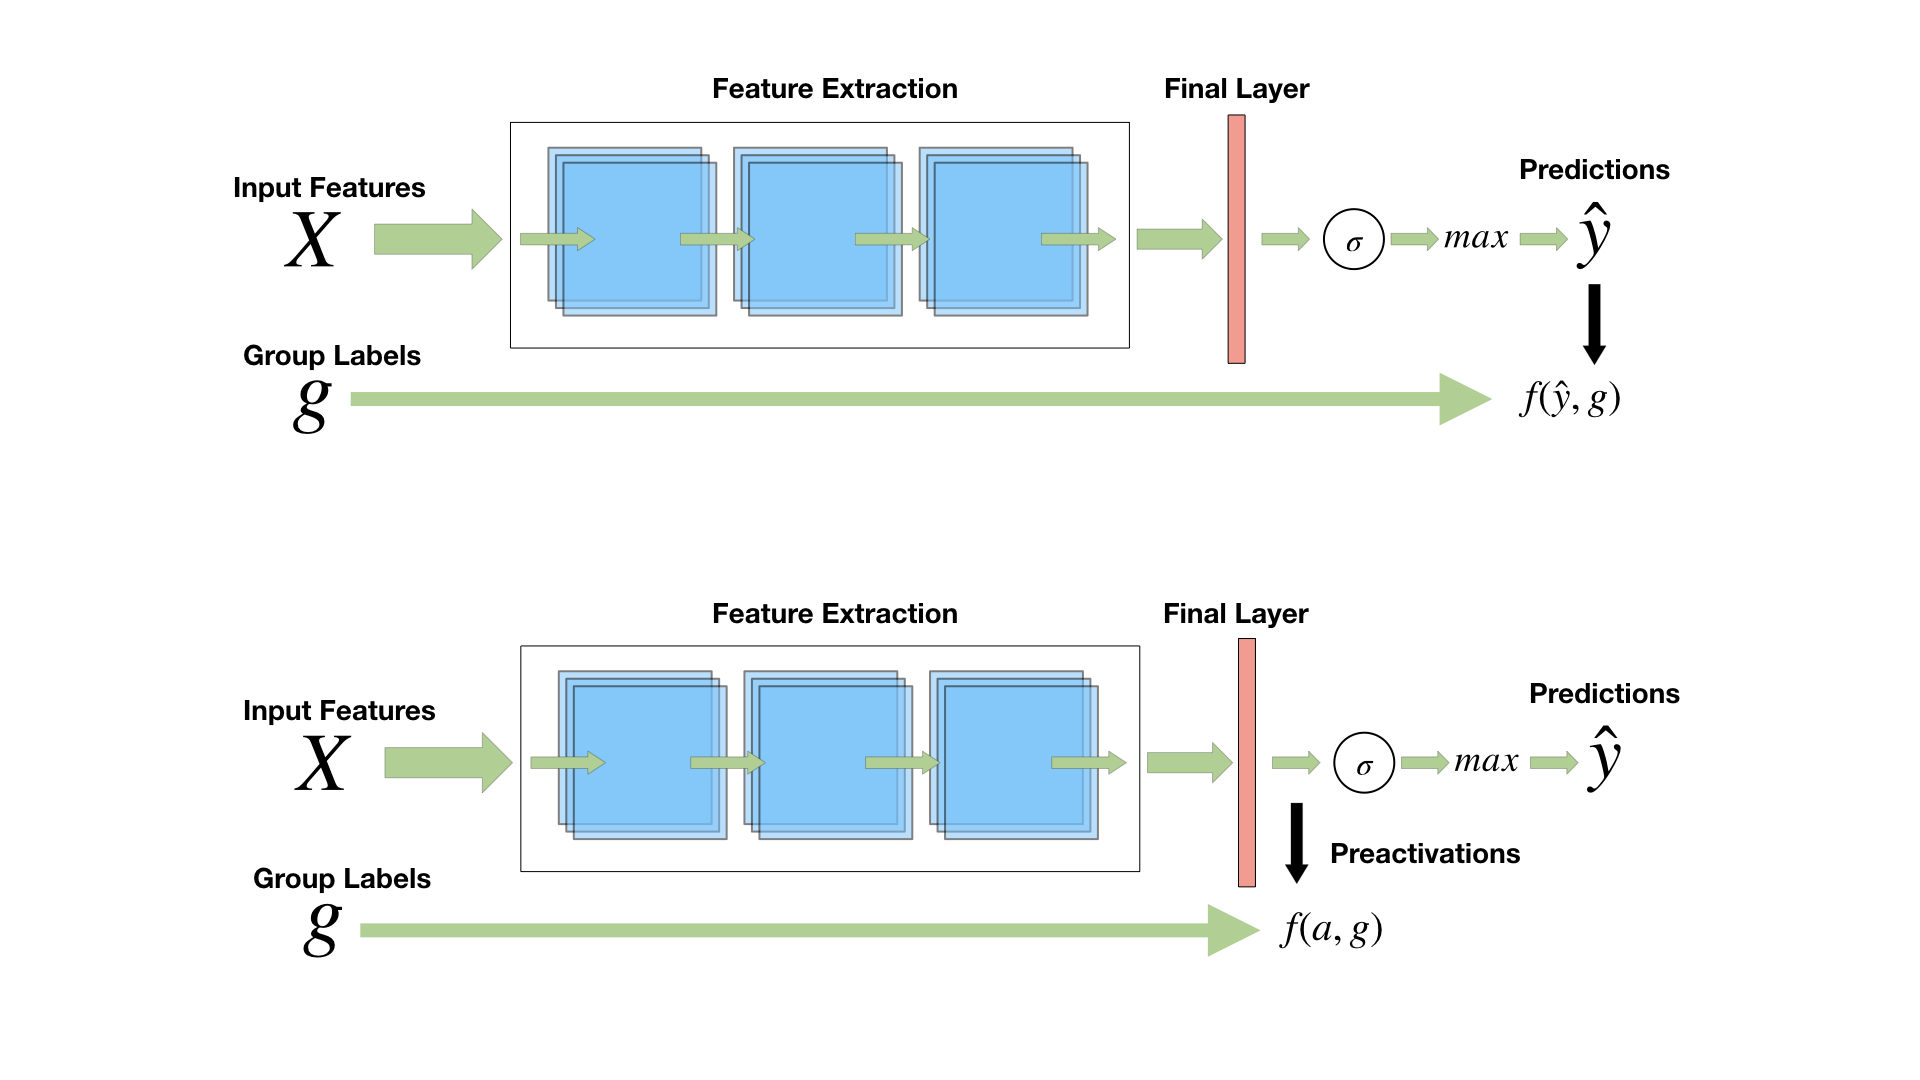
\includegraphics[trim={8cm 0 8cm 0},clip,width=\textwidth]{figs/net_diff.png}
%   \captionof{figure}{This is another figure.} \label{myfig2}
% \end{minipage}



% While gradients are now readily available, typical machine learning pipelines do not have distributions or histograms predefined at outputs which can be fed directly into our EM Loss. Applying existing binning procedures over the batch to estimate histograms will break the ability to autodifferentiate: soft thresholds are necessary at bin boundaries such that samples within a bin may move smoothly as needed. Algorithm \ref{alg:diffhist} provides a differentiable histogram implementation. Using a rectified linear relaxation allows for samples to have a continuous gradient towards neighboring bins.


% \subsection{Minimizing over Multiple Dimensions}
% {\color{red} @Ronak - shall we delete this section?}
%     -extending past simple computation
%     -minimizing DEMD: forcing distributions to become similar wrt to distance
%     -if possible, would lead to another, fast, way to push distributions together/towards "barycenter"

%     minimizing GEM
%     at first does not seem different from existing wass bary approaches
%     requires differentiating through distance computation, updating many times
%     -however particular algorithm of above leads to direct identification of gradients
%     -no backwards derivations/complex derivatives necessary

% \subsection{The dual linear program and back propigation}
% {\color{red}@Ronak - do you want to place backprop comments here or below?}
% The above allows for a direct plug in to existing frameworks. By manually defining the backward pass using the dual variables, the forward pass can be written explicitly and the dual variables stored for backpropagation. 

% \ronak{Will add algorithmic block detailing forward/backward, example in loss/reg formulation}


% Procedure 1:
% \begin{enumerate}
%     \item Given a trained model $\theta$,
%     \item compute the d-EMD distance for all groups
%     \item identify the groups with maximal ``unfairness" via the hull in \eqref{eq:dEMD}.
%     \item Take a coordinate step in reducing the gap.
%     \item Repeat.
% \end{enumerate}


%% This declares a command \Comment
%% The argument will be surrounded by /* ... */
% \SetKwComment{Comment}{/* }{ */}
% \begin{algorithm}
% \caption{Algorithm Pseudocode}\label{alg:main}
% \KwData{$X, Y, G$, algorithm $f$ that learns $\theta$}
% \KwResult{Fair model $\theta$}

% \KwFor{stopping cond} {
%     $\theta_{next} = f(X,Y, G_{prev}, \theta_{prev})$\;
%     Compute EMD for all $G$.\;
%     $G_{next}$ = Select maximally unfair groups via \eqref{eq:floormin}\;
%     $\theta_{prev} = \theta$\;
%     $G_{prev} = G_{next}$\;
% }
% \end{algorithm}